\documentclass[10pt,a4paper]{article}
\usepackage[margin=2cm]{geometry}
\usepackage{amsmath,amssymb,graphicx,caption,float,hyperref,xcolor}
\hypersetup{colorlinks=true,linkcolor=blue!50!black,urlcolor=blue!50!black}
\captionsetup{font=small,labelfont=bf}
\graphicspath{{../../figures/}}
\title{\vspace{-1.2cm}\textbf{What carries the persistence}\\[2pt]
\large Simulation 2, \texttt{task003-symmetric} and \texttt{task003-nosolution}}
\author{Step 3 of the key-phenomena study (Campaign B); 20 October 2026}
\date{}
\begin{document}
\maketitle
\vspace{-1cm}

\paragraph{Run.} \texttt{results/simulation\_2/2026-10-20\_sim2\_persistence\_branches}: both setups, $\rho = 0.25$
(no relaxation in step 1) and $0.75$ (partial relaxation), $q = 6$, $q_c = 12$, $\lambda_c = 1$, gate on, $B = 30$,
$W = 48$, 1{,}000 paired episodes, to $t = 130$ (32 settings, 3.9 GB). From $t = 30$, when the controller stops,
four rules (new simulator setting \texttt{post\_stop\_mode}), each with its own silent arm:
\emph{normal}; \emph{no reading or posting}; \emph{frozen board} (agents read only the posts on the board at $t = 30$
and post nothing); \emph{controller-only facts removed} from every memory and from the board. All four are identical
to normal up to $t = 30$ (keyed random streams; tested), and normal reproduces the earlier runs exactly up to
$t = 40$. $\delta(t)$: the paired effect on the A2 vote share. Bands: 95\% intervals.

\begin{figure}[H]
\centering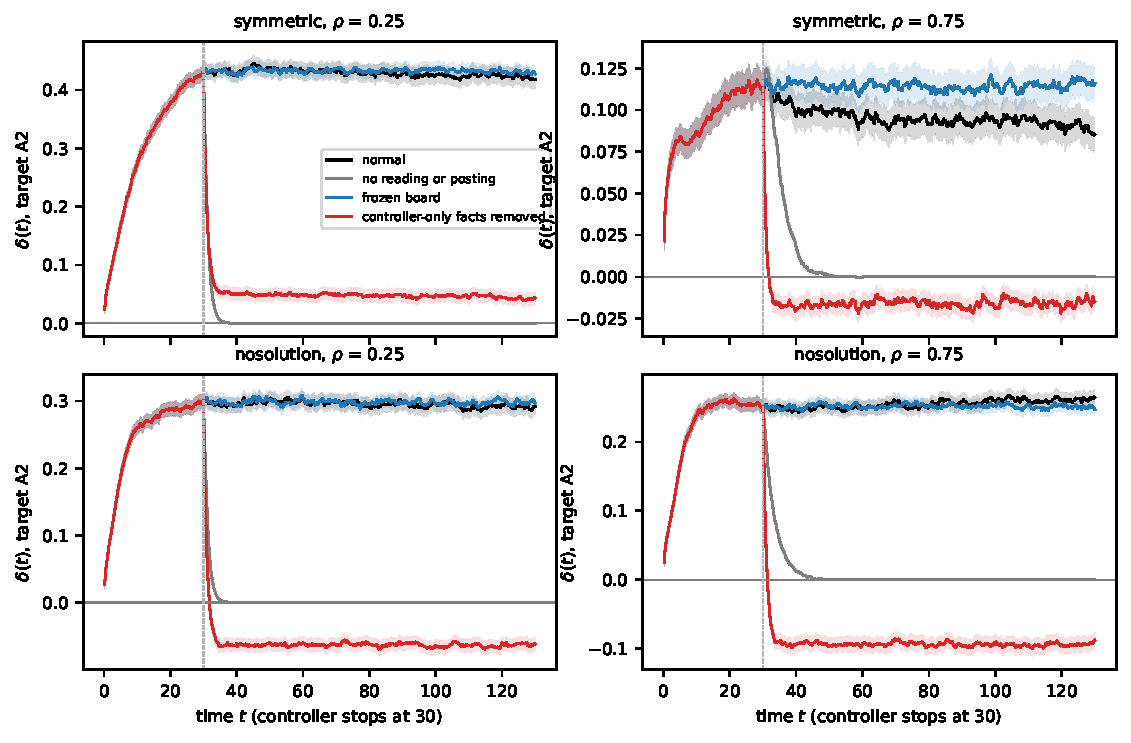
\includegraphics[width=0.95\linewidth]{step3_fig1_delta.pdf}
\caption{$\delta(t)$ for the four post-stop rules; one panel per setup and memory.}
\end{figure}

\begin{itemize}\itemsep1pt
\item Normal: no relaxation over 100 time units at $\rho = 0.25$ (nosolution 0.30 $\to$ 0.29, symmetric 0.43 $\to$
  0.42 at $t = 130$) or in nosolution at $\rho = 0.75$ (0.25 $\to$ 0.26); only symmetric $\rho = 0.75$ drifts slowly
  (0.11 $\to$ 0.085). That is over 40--200 half-lives of an unread fact.
\item No reading or posting: the effect vanishes, with half-times 1 ($\rho = 0.25$) and 2.5--5.5 ($\rho = 0.75$) time
  units, as memories empty to the prior. Passive memory does not carry it.
\item Frozen board: the effect is kept in full (0.30, 0.43, 0.25, 0.12 at $t = 130$). New posts are not needed;
  re-reading the board as it was at $t = 30$ is enough.
\item Controller-only facts removed: the effect collapses within 1 time unit (half-times 0.5--1) to a small residual,
  negative in nosolution ($-0.06$ at $\rho = 0.25$, $-0.09$ at $0.75$), $+0.04$ and $-0.015$ in symmetric.
\item The residual equals the indirect part of step 2 (belief shift after removal at $t = 40$ against step 2's
  indirect part at $q = 6$): nosolution $-0.022$ / $-0.021$ and $-0.083$ / $-0.089$; symmetric $+0.019$ / $+0.028$ and
  $-0.022$ / $-0.024$.
\end{itemize}

\begin{figure}[H]
\centering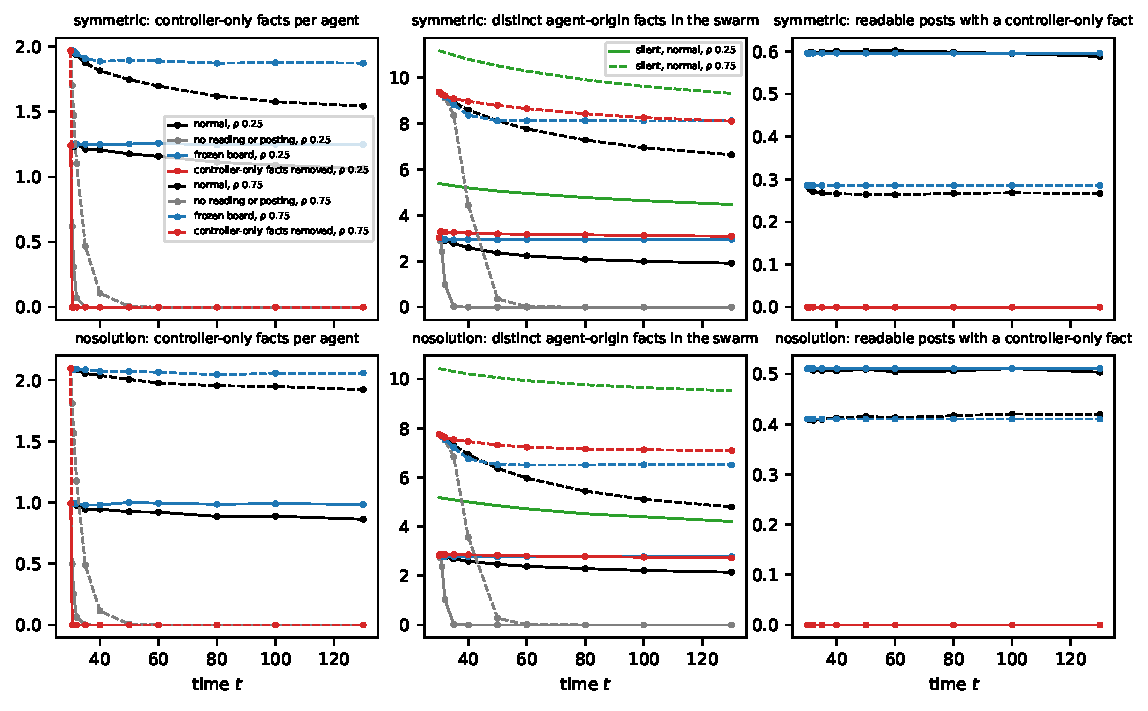
\includegraphics[width=0.95\linewidth]{step3_fig2_carriers.pdf}
\caption{False arm over time, per rule ($\rho = 0.25$ solid, $0.75$ dashed): controller-only facts per agent;
distinct agent-origin facts held by anyone (green: silent arm, normal); share of the 48 newest posts that carry a
controller-only fact (with no reading or posting nobody reads them).}
\end{figure}

\begin{itemize}\itemsep1pt
\item Under normal rules the controller-only facts stay in memory (nosolution $\rho = 0.25$: 0.99 $\to$ 0.86 per agent
  at $t = 130$) and on the board (27--60\% of readable posts throughout): agents keep reposting them.
\item Agent-origin coverage keeps falling in every normal arm, silent included (nosolution $\rho = 0.25$: 5.2 $\to$ 4.2):
  a fact nobody holds or posts is lost for good. The false arm loses more.
\item After removal the false arm still holds fewer agent-origin facts than the silent arm (nosolution $\rho = 0.75$:
  7.1 against 9.5), yet the effect is gone: the missing agent evidence alone does not sustain it.
\end{itemize}

\paragraph{Conclusion.} The persistence is carried by the controller-only facts themselves, kept alive by agents
re-reading and reposting them. It needs neither the controller nor new posts, and it is not passive individual
memory. Removing those facts removes the effect, leaving only the shift in which agent facts were kept.

\end{document}
